\chapter{Testing}
\label{sec:testing}
In this chapter we will be talking about the different techniques that we have employed to test the different aspects of the system.
We will first be talking about the different kind of unit tests that we have written.
These tests provide a basic code coverage.
After this we will be talking about what kind of integration tests we have performed to ensure the connection between the different components.
Lastly we will be talking about the requirement tests that were performed, to test if we achieved our goals.

\section{Testing methods during the implementation phase}
During the implementation phase, we already started with testing.
Because the system was not completed during this phase, only parts of the system could be tested.
We have tested each feature with unit tests, see Section~\ref{sec:unit_test}.
We also performed integration test during the implementation phase, see Section~\ref{sec:integration}

\subsection{Unit testing}
\label{sec:unit_test}
During the implementation phase a feature is only complete when it is fully tested.
This is done by test from the programmer while running the system, but also done by running automated tests.
These automated tests are required for achieving a good code coverage and for ensuring the code to function appropriately.
The tests that are written for other features will be always run before the feature has been merged.
This ensures that other features that may change the function of the code does not let the tests fail.
So all the features that were already in the system will still function even after the merging of the new feature.

In figure~\ref{testresulttrenddev} you can see the increasing amount of tests that increase with each pull request that has been merged with the development branch.
\begin{figure}[H]
    \centering
    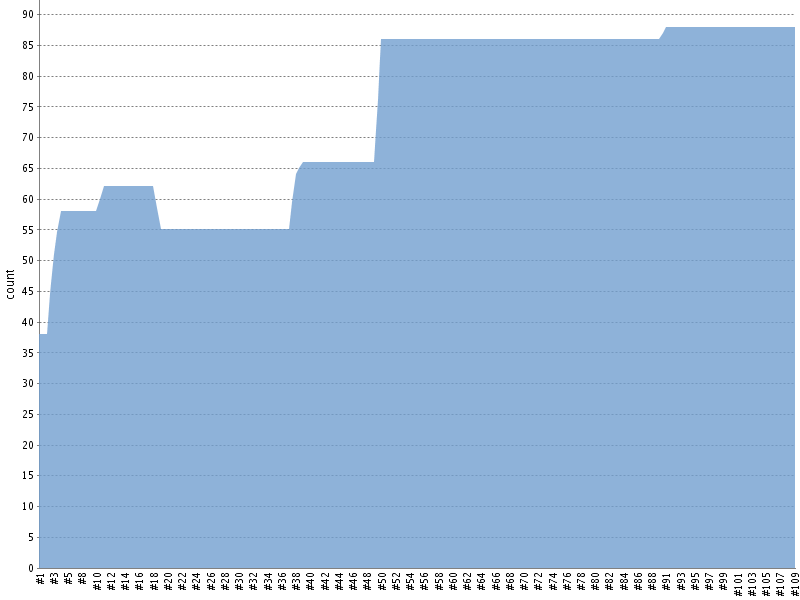
\includegraphics[width=\textwidth]{images/TestresultTrendDev2}
    \caption{Amount of tests per build}
    \label{testresulttrenddev}
\end{figure}

In figure~\ref{testresulttrendpullrequest} you can see the increasing amount of tests of the different pull requests that have been made.
In this image you can clearly see that when sometimes when a new feature is added, some tests start to fail.
Due to our continuous integration we could spot the errors early and make sure that they are fixed before merging with the development branch.

\begin{figure}[H]
    \centering
    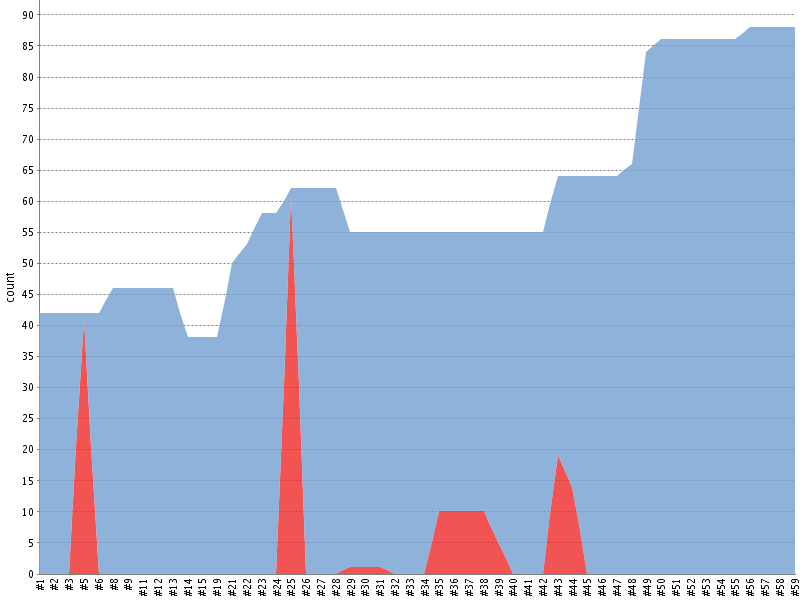
\includegraphics[width=\textwidth]{images/TestresultTrendPullRequests}
    \caption{Amount of tests per build of a pull request}
    \label{testresulttrendpullrequest}
\end{figure}

Figure~\ref{testresulttrendpullrequest} shows how not every pull request is without errors.
All of these errors first had to be resolved before the pull request could be merged.\\

Figure~\ref{codecoveragetrenddev} depicts the code coverage achieved by the tests.
The goal is to have the code coverage percentages to be around a certain percentage during the entire implementation.
One could argue that a 100\% code coverage is desired, but some features are quite trivial and don't need a 100\% code coverage.
Next to this is the fact that some plugins, in our case the eBean plugin, generates code for classes.
This generated code is not something we need to test since it is not written by us.\\

\begin{figure}[H]
    \centering
    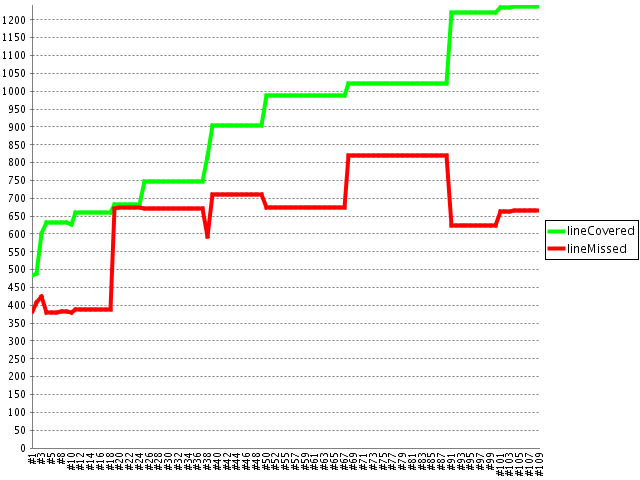
\includegraphics[width=\textwidth]{images/CodeCoverageTrendDev2}
    \caption{Code coverage trend for the development branch}
    \label{codecoveragetrenddev}
\end{figure}

We also underestimated the complexity of some features and thus did not wrote the tests for all cases with the first pull request of those features.
In that first basic implementation some of the cases were already implemented in part of the system but not actually called upon and made available from the front end.
We thus decided to first create a pull request for a basic version and thus split up the amount of changes.
Later, when the feature was further implemented, we added tests that would test these extra cases.

\subsection{Integration testing}
\label{sec:integration}
Every time a pull request was made, the changes were checked by a member of the team that did not make the pull request.
This ensured that the changes made reflected the feature that was selected to be implemented.
The member of the team to check the code asked questions about some changes and checked if complex functions could be made more efficient.
Although we use checkstyle and findbugs to perform code analysis, they did not find everything.
So there is much value to achieve with a member of the team checking the code.

In figure~\ref{pullrequest-example} you can see an example of a pull request and how a team member commented on a part of the code.
The requesting team member responded on the issue and argued why he choose the implementation.

\begin{figure}[H]
    \centering
    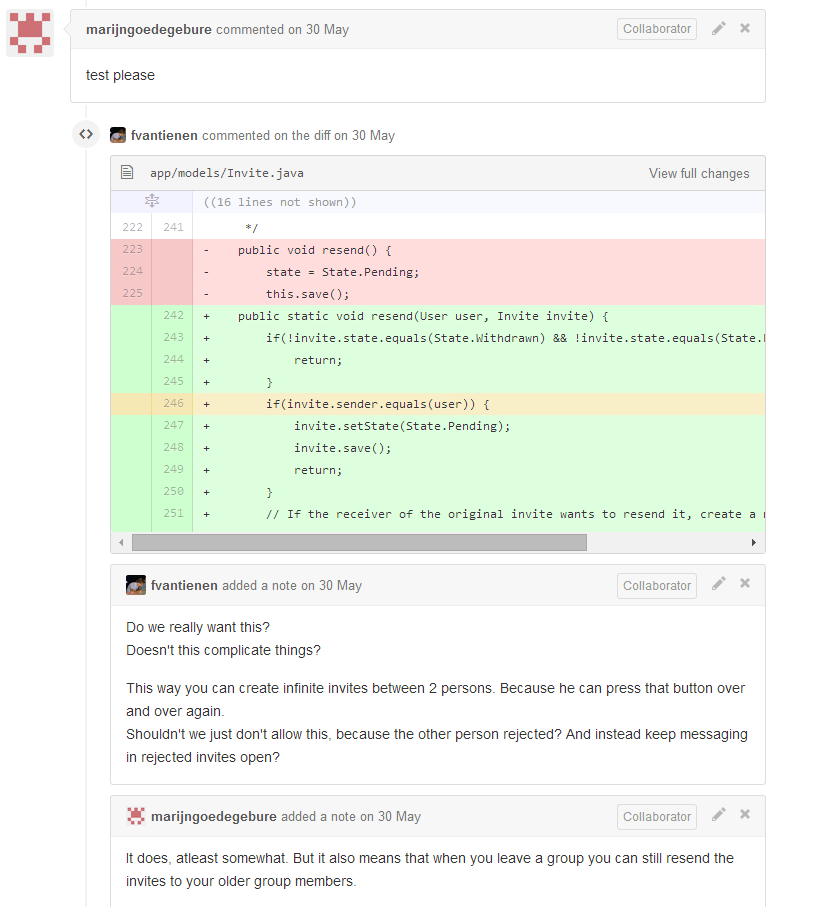
\includegraphics[width=\textwidth]{images/pullrequest-example1}
    \caption{An example of a pull request comment and reply.}
    \label{pullrequest-example}
\end{figure}

For an overview of the pull request and the comments that were made, you can find more information on the following website:
https://github.com/florisverburg/pm-impl/pulls

\section{Testing methods after the implementation phase}
The testing of the entire system is done after the implementation phase has been completed.
This is partly done by checking if the final product matches the requirements set.
It is also done by letting the target audience use the system and document the findings.
We will start with describing the user tests.

\subsection{User test}
The purpose of the user test is to test the system without the limiting factors of a development environment.
The system will be tested for his robustness in the different kinds of input a user can generate.
The test also let's the user make extensive use of the interface that we provided.
Any errors will be revealed by the user's interaction.
If the tester finds anything unclear he can comment on that in the appropriate text boxes provided in the survey, see Appendix~\ref{app:survey}.

To test the system we will be defining the people that are valid testing subjects and how we documented the various aspects of the test.

\subsubsection{The user}
We define a valid subject for our user test as a person that is part of the target audience (which we already defined in an earlier chapter).
The user should also be unfamiliar with the system.
We will focus our user test on the students, since they will be the biggest group of users of the system.

\subsubsection{The test}
The user will be asked to test different functionalities which we will define beforehand.
The functionalities that are included in the survey for testing are the following:
\begin{itemize}
\item Registration
\item Logging in
\item Register to practical using url
\item Viewing the practical that they registered to
\item Invite other student to join your practical group
\end{itemize}
We hand the user a document which lists the different actions that we want the user to do.
Before and after the test we let the user fill in a survey.
The survey at the start is about who the user is and the survey at the end is about what they thought of the system.
To easily process the responses that we receive, we have used a google form.
In this Google form we have combined the survey and the step by step action plan for the tester.
The Google form document can be found in Appendix~\ref{app:survey}.

\subsubsection{The user test results}
The user test was conducted during two days and provided us with some interesting comments about the system.
In this section we will give a brief summary of the results of the survey and what we can do with this feedback.\\

As you can see in the complete survey that is in Appendix~\ref{app:survey}, we started the test with a few basic questions.
First three questions about our demographic:
\begin{itemize}
\item What is your age?
\item What is your occupation?
\item Do you know what a MOOC is?
\end{itemize}

Both questions gave results that we expected.
As you can see in Figure~\ref{demographic_chart}.

\begin{figure}[H]
    \centering
    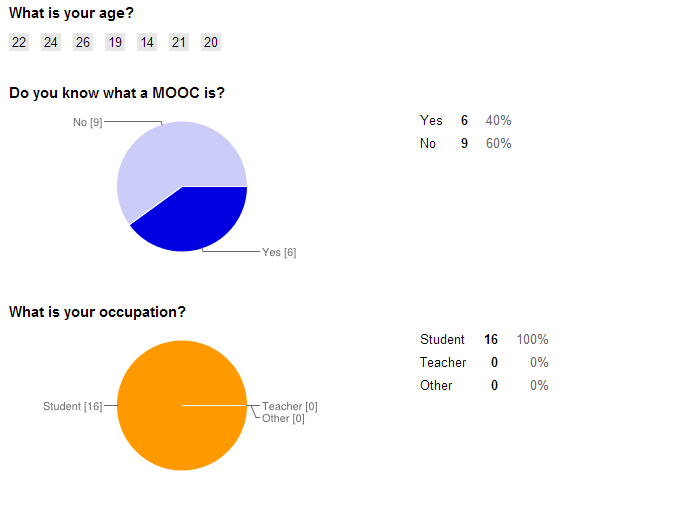
\includegraphics[width=\textwidth]{images/demographic_chart}
    \caption{Demographic questions}
    \label{demographic_chart}
\end{figure}

The image above shows us that the people that were questioned were all students and between the appropriate age to be in our target audience.

More surprising is the amount of people that knew what a MOOC is.
We thought this to be much more than the figures shows.

After the occupation question there was a split up in the survey.
Students and teachers would be given different questions from there on.
The other that could have been filled in would have submitted the survey directly.

The student part of the survey gives us more information about our demographic, as can be seen in figure~\ref{student_demographic_info}.\\
\begin{figure}[H]
    \centering
    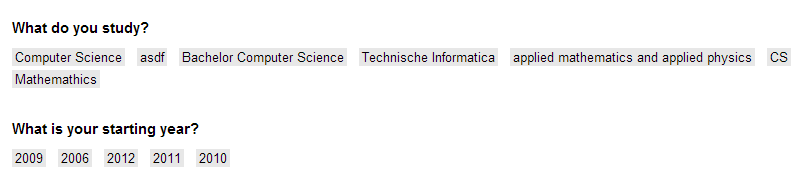
\includegraphics[width=\textwidth]{images/student_demographic_info}
    \caption{Student demograhpic info }
    \label{student_demographic_info}
\end{figure}

We did not have any respondents that were teachers or "others" so we do not have any data on the other part of our target audience.
Having more time for an extended survey would definitely give more information about the demographic of our target audience.

After the first survey, the participant had to perform a number of actions on the system.
After each action there were a couple questions asked.
One of these questions was always about possible improvements.
This was asked to give the participant the possibility to give suggestions.\\
The first action to be performed was the registration and logging in to the system.
In figure~\ref{register_login_chart} you can see the answers to these questions:\\
\begin{figure}[H]
    \centering
    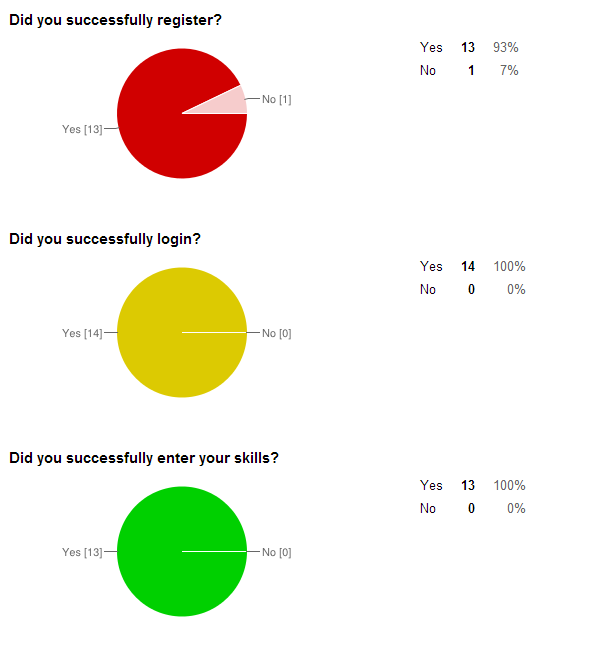
\includegraphics[width=\textwidth]{images/register_login_chart}
    \caption{Register and login success rates}
    \label{register_login_chart}
\end{figure}

The charts shows a positive reaction to the registration and the log in parts of our system.
Almost all of the participants succeeded in registering and logging in.

There were, however, some comments on how some parts had errors in them or how some parts were unclear. We made a list of these suggestions:
\begin{itemize}
\item Require fields tooltips sometimes align wrong
\item Email activation link was not clickable
\item The scale for a skill could be something different then from 1 to 10, since most people do not tend to give themselves a bad "grade".
\item Send an email with more text, this way people become more involved
\item There needs to be more incentive to enter your skills
\item The slider value is not correctly updated
\end{itemize}

Each of these suggestions highlight some aspect of the system that needs to be looked at.
All of these things can be used in future improvements of the system.
This might also be things to look into during the week between the final report and the presentation.

The next part of the test was the registration to a practical using an url and viewing the freshly registered practical.
The first couple of questions were about whether the functionality worked and whether the participant had any suggestions on the functionality.
The second part was focussed on the recommendations.

The charts of the first part can be seen in figure~\ref{register_practical_chart}\\
\begin{figure}[H]
    \centering
    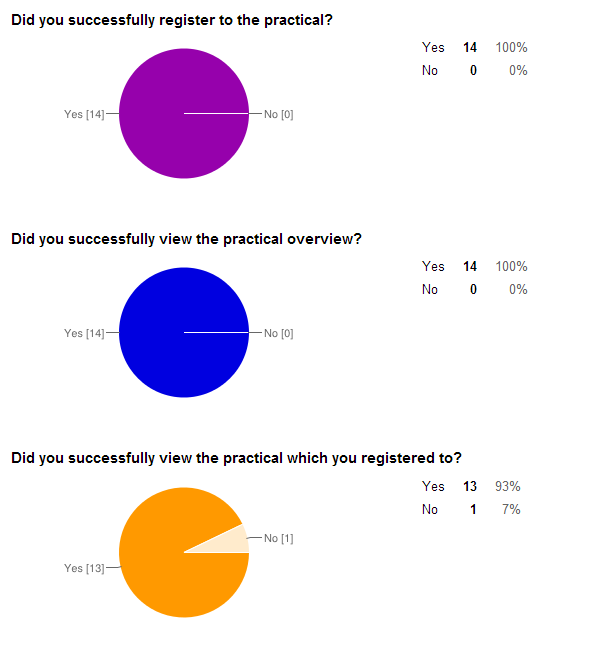
\includegraphics[width=\textwidth]{images/register_practical_chart}
    \caption{Practical registration and viewing success rate}
    \label{register_practical_chart}
\end{figure}

The charts indicate that almost all of the participants have successfully registered to the practical and have successfully viewed the appropriate practical.\\

The suggestions indicate that there are some important improvements that can be done to make the system more accessible.
The list of suggestions and remarks is as follows:
\begin{itemize}
\item No explanation of the purpose of the practical page
\item A notice of a successful registration
\item Unclear why there are links to other practical groups
\item Unclear what the purpose is of the invitations
\item Show names instead of practical groups
\item Explanation of the recommended skills
\end{itemize}

We also noticed that the fact that some students were unfamiliar with MOOC's played a role in their ability to deduce the meaning of the numbers on the page and the meaning of the system.
Since the system will have to be used by all kinds of users, we need to improve vastly on the interface and the explanation of what the system does.
There are many possibilities for improving the system and we will have to look into the different possibilities to select the best one.

The chart about the recommendations can be seen in figure~\ref{recommendations_chart}, followed by the suggestions and remarks.\\
\begin{figure}[H]
    \centering
    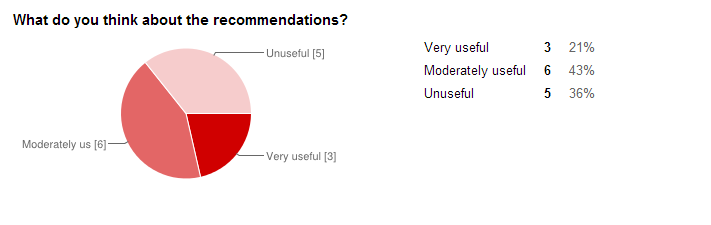
\includegraphics[width=\textwidth]{images/recommendations_chart}
    \caption{Recommendation usefulness rating}
    \label{recommendations_chart}
\end{figure}

\begin{itemize}
\item Explain what is it recommending me
\item For who are the recommendations?
\item What are the recommendations based on?
\item What is meant by recommendations? Are these my targets?
\item What do the values mean and what do I do with it?
\end{itemize}
This chart is combined with the suggestions and remarks let's us conclude that there should be a lot more information about the workings of the recommendations.
People who will work with the system will require that information to believe that the recommendations are really working in their favour.\\

The last feature to test was the invitation of another student to join your practical group.\\
Figure~\ref{invite_chart} shows the success rate of the participants.
\begin{figure}[H]
    \centering
    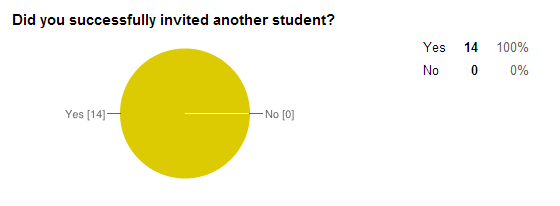
\includegraphics[width=\textwidth]{images/invite_chart}
    \caption{Invite success rate}
    \label{invite_chart}
\end{figure}

The figure shows that the interface for inviting another student is working correctly.
The suggestions and remarks are mainly about the participants how the invitation correlate to the practical groups:
\begin{itemize}
\item See other person's name and skills without going to a different page
\item Invited practical group $\#$14 but in my overview it said that I invited Peter de Jong
\item Showing the skills instead of the group names might be more convenient
\item Addition of a communication skill to improve the selection criteria
\item Should a user start being in a group?
\end{itemize}

The comments raise an interesting point about whether we should change the user being in a group from the start or that a group should be created when an invite is accepted.
It makes sense to do so, but we have multiple ways of changing this.
We can either only change the front end representation or change the way accepting invites work.
Both quite easily to do and worth changing.

The last part of the final survey asked a very important questions concerning the role of the recommendations:
What did you think about the usage of recommendations to suggest possible group members?\\
\begin{itemize}
\item Cool that you provide recommendations
\item Good idea
\item This was useful. With these recommendations you did not have to scan through all the people
\item Great addition to courses! Not quite sure whether or not the using of recommendations to create the overall optimal group composition is the best way. A group with members of equal skill might be a better solution
\end{itemize}
The comments about the recommendations were great.
It is nice to know that students appreciate the goal of the system.\\

\subsubsection{User test reflection}
The user test gave us the opportunity to test some essential parts of the system by open minded participants who are part of our target audience.
They provided us with detailed feedback on the different aspects of the system.
The user test did not gave us the possibility to completely test the invite system.
To have this part tested by our target audience we need a different kind of test.
A test that runs over the course of a week in which multiple users try to use the system at multiple times.
Such a test would be a great way and quite necessary to have the system tested before it could be used in a real MOOC.

The feedback that we collected with the user test gives us some great improvements that we can consider for feature work.
We will talk more about feature work after the conclusion.

\subsection{Requirements test}
In chapter 2 we define global goals, global requirements and detailed requirements.
We will go into the detailed requirements in this chapter, the other two will be discussed in the conclusion.
In the detailed requirements section we divided the requirements into four categories following the MoSCoW-model.
The categories are:
\begin{itemize}
\item Must have, classifies as requirements that have to be in the final product, without these requirements the product would not be usable.
\item Should have, these requirements are desired, but without these the product is usable.
\item Could have, these requirements will be implemented if there is enough time.
\item Would have, these requirements will not be looked into for this project, but can be interesting for a feature project.
\end{itemize}

Following the MoSCoW-model we can now say that we should at least have all of the must have requirements implemented or a good reason why we have not.
We will first list the must haves that we have not implemented and why not.
Secondly we look at which should have requirements we did and which should have requirements we did not implement.
Using this, we will determine the progress we made during the project and if we correctly used the MoSCoW-model.
The could and would have requirements will be discussed in the future work section.

\subsubsection{Must haves}
In the following table we listed the must have requirements that were not met.

\begin{tabular}{ | p{12cm} | p{2cm} | }
\hline
\textbf{Requirement} & \textbf{MoSCoW} \\ \hline
\multicolumn{2}{|p{14cm}|}{\textbf{Actor 1: MOOC participant}} \\ \hline
The potential participant (anyone who visits the site) must be able to view the different MOOCs without registering or logging in. & M \\ \hline
The participant must be able to inform him/herself about the usage of the application without registering or logging in. & M \\ \hline
\end{tabular}

During the user test we noticed that the two must haves that we did not implement, were quite essential to the system.
Due to the nature of the project, a proof of concept, we focussed more on implementing interesting features than making the system more understandable.
So as a proof of concept point of view these requirements were probably more should haves than must haves, but from a user point of view these requirements were far more important than we have treated them.


\subsubsection{Should haves}
In the following section we will show a list of should have requirements that we have implemented and we discuss why we have chosen for these requirements to be implemented.
Following, we will shortly discuss the requirements that we have chosen not to implement and why we have not implemented these requirements.

We will first start with the list of requirements that have been implemented:

\begin{tabular}{ | p{12cm} | p{2cm} | }
\hline
\textbf{Requirement} & \textbf{MoSCoW} \\ \hline
Users should be able to enter the basic user information, like: country, age, short description, skills, education, a picture and personality traits. & S \\ \hline
The participant should be able to ask a currently existing group if he can join them. & S \\ \hline
The participant should be able to use their LinkedIn profile to log in to the application. & S \\ \hline
In case the participant already has an account, the participant should be able to add the course to his profile using the teachers url. & S \\ \hline
The participant should be able to receive an invitation from a group. & S \\ \hline
The participant should be able to accept the invitation from a group. & S \\ \hline
A group should be able to view a possible group member. & S \\ \hline
A group should be able to invite a possible group member to join their group. & S \\ \hline
A group should be able to accept an request from a participant to join their group. & S \\ \hline
The algorithm uses basic user provided data (e.g. education, preferences) to build up a profile for a course participant. & S \\ \hline
The algorithm can calculate whether two people will be good practical partners using the basic user provided data. & S \\ \hline
The algorithm can return a possible practical partners using the basic user provided data. & S \\
\hline
\end{tabular}

Following the goal to create a proof of concept we implemented the should haves that focus on facilitating a more complete proof of concept.
We implemented a lot of the recommendation algorithm should haves, since it would make the proof of concept a lot better.

Next to this is the invitation system.
While setting up the invite system, we kept in mind that both single students as groups of students will be using this system.
This helped with formulating a system where single students can invite other single students and other groups, and where groups can invite other single students and groups.
This gives the single students (and groups) complete freedom in creating their practical groups.

The requirements that we have chosen not to implement are mainly requirements about the teacher's part of the system.
Due to the goals of the project we thought these requirements to have a lower priority and not be very important to the proof of concept.
These requirements will become interesting when the implementation continues and is focussed on usage of the system.

\subsubsection{Requirements test conclusion}
As we can conclude from the analysis done in the previous sections, we can definitely say that we made a good estimation of the scope of the project.
Due to the time and an underestimation of the importance, we did not manage to complete all the must haves.
The two must have requirements that still need to be done are quite easy to implement and should be at the top of the list of things to be done.
Although we failed to implement all the must haves before the delivery of this report, we did managed to implement a lot of should haves.

\section{Software Improvement Group Feedback}
\subsection{Intermediate feedback}
\subsection{Improvements}
\subsection{Final feedback}


